% Это основная команда, с которой начинается любой \LaTeX-файл. Она отвечает за тип документа, с которым связаны основные правил оформления текста.
\documentclass{article}

% Здесь идет преамбула документа, тут пишутся команды, которые настраивают LaTeX окружение, подключаете внешние пакеты, определяете свои команды и окружения. В данном случае я это делаю в отдельных файлах, а тут подключаю эти файлы.

% Здесь я подключаю разные стилевые пакеты. Например возможности набирать особые символы или возможность компилировать русский текст. Подробное описание внутри.
\usepackage{packages}

% Здесь я определяю разные окружения, например, теоремы, определения, замечания и так далее. У этих окружений разные стили оформления, кроме того, эти окружения могут быть нумерованными или нет. Все подробно объяснено внутри.
\usepackage{tikz}
\usepackage{tcolorbox}
\usepackage{mathrsfs}
\usepackage{amsmath}
\usepackage{environments}
\newcommand{\Q}{\mathbb{Q}}
\newcommand{\N}{\mathbb{N}}
\newcommand{\Z}{\mathbb{Z}}
\newcommand{\R}{\mathbb{R}}
\newcommand{\Li}{\mathscr{L}}
\newcommand{\hh}[1]{\boxed{\rule[-0.9cm]{0cm}{2cm}#1}}
\newcommand{\llo}[1]{\boxed{\rule{0.5cm}{0cm}#1\rule{0.5cm}{0cm}}}
\newcommand{\mm}[1]{\boxed{\rule[-0.4cm]{0cm}{1cm}\rule{0.2cm}{0cm}#1\rule{0.2cm}{0cm}}}

% Здесь я определяю разные команды, которых нет в LaTeX, но мне нужны, например, команда \tr для обозначения следа матрицы. Или я переопределяю LaTeX команды, которые работают не так, как мне хотелось бы. Типичный пример мнимая и вещественная часть комплексного числа \Im, \Re. В оригинале они выглядят не так, как мы привыкли. Кроме того, \Im еще используется и для обозначения образа линейного отображения. Подробнее описано внутри.
\usepackage{commands}

% Потребуется для вставки картинки подписи
% \usepackage{graphicx}

% Пакет для титульника проекта
\usepackage{titlepage}

% Здесь задаем параметры титульной страницы
\setUDK{192.168.1.1}
% Выбрать одно из двух
% \setToResearch
\setToProgram

\setTitle{Нейросеть с нуля}

% Выбрать одно из трех:
% КТ1 -- \setStageOne
% КТ2 -- \setStageTwo
% Финальная версия -- \setStageFinal
%\setStageOne
%\setStageTwo
\setStageFinal

\setGroup{211}
% Сюда можно воткнуть картинку подписи с помощью \includegraphics[scale=0.2]{2023-02-07 22.29.16.jpg}
% (scale подбирается индивидуально для конкретной картинки)
%\setStudentSgn{\includegraphics[scale=0.02]{sign.jpg}}
\setStudent{Д. А. Сорокин}
\setStudentDate{05.02.2023}
\setAdvisor{Дмитрий Витальевич Трушин}
\setAdvisorTitle{доцент, к.ф.-м.н.}
\setAdvisorAffiliation{ФКН НИУ ВШЭ}
\setAdvisorDate{12.06}
\setGrade{11}
% Сюда можно воткнуть картинку подписи с помощью \includegraphics[scale=0.2]{<имя файла>}
% (scale подбирается индивидуально для конкретной картинки)
%\setAdvisorSgn{\includegraphics[scale=0.5]{tru.png}}
\setYear{2023}


% С этого момента начинается текст документа
\begin{document}

% Эта команда создает титульную страницу
\makeTitlePage

% Здесь будет автоматически генерироваться содержание документа
\tableofcontents

% Данное окружение оформляет аннотацию: краткое описание текста выделенным абзацем после заголовка
% \begin{abstract}
% Текст аннотации. Здесь кратко в два-три предложения описываем, что происходит в работе.
% \end{abstract}

\newpage

\section{Введение}
В современном информационном обществе нейронные сети стали одной из наиболее востребованных и перспективных областей искусственного интеллекта. Нейронные сети используются для решения разнообразных задач, включая распознавание образов, классификацию данных, прогнозирование и генерацию контента. Они являются основой многих инновационных технологий, таких как автономные автомобили, рекомендательные системы, медицинская диагностика и многое другое.

Целью данного курсового проекта является создание простой имплементации нейронной сети с использованием основных концепций и алгоритмов, лежащих в ее основе.

Результатом является написанная на языке C++ библиотека, предоставляющая функционал для создания и обучения нейронных 
сетей при помощи алгоритма градиентного спуска.

\section{Основные идеи нейронных сетей:}
Структура нейронной сети пришла в програмирование из биологии, где 
она описывает строение нервной ткани. 

Упрощенно один нейрон можно представить следующим образом:
\begin{align}
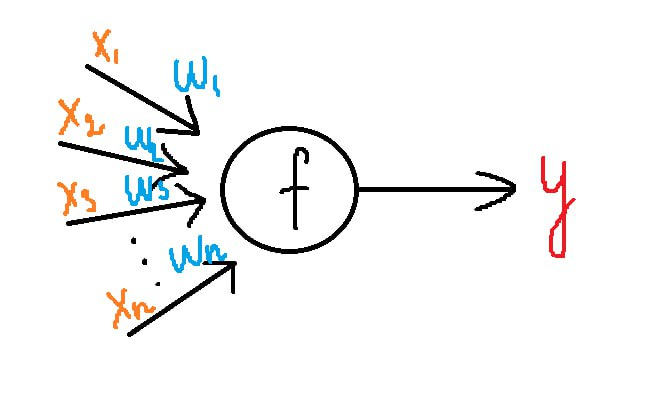
\includegraphics[scale=0.5]{neuron.png}
\end{align}

У него есть n входящих связей от других нейронов, при этом
для каждой связи определен её вес, и один выходящий канал. 
Нейрон принимает данные по входящим связям и передает вычисленное значение дальше
$f(x_1, ... x_n) \to y_{predicted}$.

Вместе нейроны образуют сеть, где каждый нейрон связан с другими. В нашей модели мы будем считать, 
что нейроны идут по слоям - каждый слой связан с предыдущим и следующим:
\begin{align}
    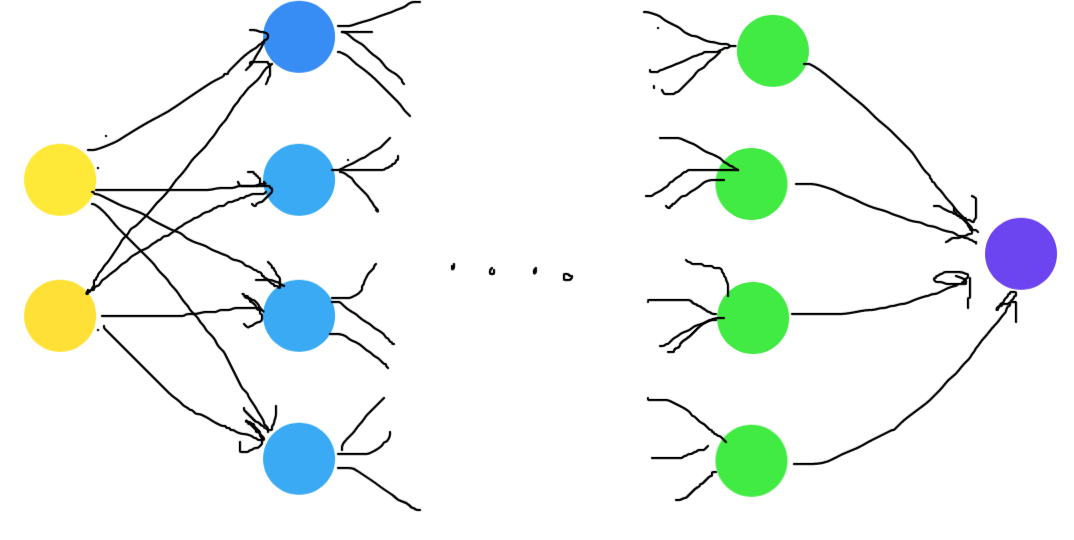
\includegraphics[scale=0.5]{neuronNetwork.png}    
\end{align}
Процесс обучения можно описать как коректировку весов в нейронах, для получения лучшего результата.

Теперь опишем это математическим языком:

Каждый уровень сети представим в следующем виде:
\begin{align}
    \sigma(A \times \begin{bmatrix}
        x_1\\
        x_2\\
        x_3\\
        ...\\
        x_n
    \end{bmatrix}
    + b)
\end{align}
\begin{itemize}
    \item Внутренние параметры слоя - это $A \in R^{n\times m}, b \in R^{n}$, обозначим их за $\theta$
     и нелинейная функция $\sigma$.
\end{itemize}
Рассмотрим алгоритм обучения на примере задачи предсказания стоимости дома на основе некоторых числовых параметров(таких как площадь квартиры, высота потолков etc).
У нас есть данные из реального мира про некоторые квартиры с известными параметрами и ценой, мы хотим с помощью сети предсказывать
цену квартиры по заданным параметрам.

Тут же встает вопрос как оценивать предсказания нашей сети, для этого введем функцию потерь, 
которая является дифференцируемой функцией расстояние на пространстве векторов ответов - $\Li(y, F(x)) \to R$, где $F(x)$ - результат нашей сети.
Теперь наша задача звучит как минимизировать функцию
\begin{align}
    \Li'(X, Y) = \frac{1}{n}\sum_{i=1}^{n} \Li(F(x_i), y_i)
\end{align}

Решать эту задачу мы будем при помощи градиентного спуска - вычислим производные $\frac{\delta}{\delta \theta_i} \Li'(X, Y)$,
где $\theta_i$ - изменяемый параметр i слоя. Зная значения градиента для каждого слоя мы вычитаем его из параметров и тем самым 
сдвигаемся в сторону локального минимума функции потерь. Подробное описания вычисления градиента приведено ниже.
\section{Основные математические выкладки:}
Напомним вид нашей сети:
\begin{align}
    \R^n \underset{\sigma_1(A_1 x + b_1)}{\longrightarrow} \R^{n_1} 
    \underset{\sigma_2(A_2 x + b_2)}{\longrightarrow} \R^{n_2} ... 
    \underset{\sigma_k(A_k x + b_k)}{\longrightarrow} \R^{n_k}
    \underset{\Li}{\longrightarrow} \R
\end{align}
Обозначим $\Theta = (\theta_1, \theta_2 ...\theta_k)$ соотвественно
$F_{\Theta}(x)$ - функция всей нейронной сети. Мы хотим минимизировать
\begin{align}
    \Li' = \frac{1}{n} \sum_{i=1}^{n} \Li(F_{\Theta}(x_i), y_i)
\end{align}
А точнее необходимо найти 
\begin{align}
    \frac{\delta}{\delta \theta_j}\Li' = \frac{1}{n} \sum_{i=1}^{n} \Li(F_{\Theta}(x_i), y_i) = 
    \frac{1}{n}  \sum_{i=1}^{n} \frac{\delta \Li(F_{\Theta}(x_i), y_i)}{\delta(F_{\Theta}(x_i))} \frac{\delta F_{\Theta}(x_i)}{\delta \theta_j}
\end{align}
Компонента $\frac{\delta \Li(w, y)}{\delta w}$ не зависит от $\theta_j$.

Распищем $\frac{\delta F_{\Theta}(x_i)}{\delta \theta_j}$, для этого введем несколько обозначений:
\begin{itemize}
    \item $f_j(x) = \sigma_j(A_jx + b)$ - функия j слоя
    \item $z_{j}^{(i)}$ - значение для $x_i$, которое поступило на j слой, т.е $z_j = f_{j-1}(f_{j-2}(... f_1(x)))$
\end{itemize}    
Тогда 
\begin{align*}
    \frac{\delta F_{\Theta}(x_i)}{\delta \theta_j} = \left(\prod_{u = j + 1}^{k} \frac{\delta f_{u} (z_{u}^{(i)})}{d z_u^{(i)}}\right) \frac{\delta f_j(z_j^{(i)})}{\delta \theta_j}
\end{align*}
Тогда получаем такую формулу:
\begin{align}
    \frac{\delta}{\delta \theta_j}\Li' = 
    \frac{1}{n}  \sum_{i=1}^{n} \frac{\delta \Li(z_k^{(i)}, y_i)}{\delta(z_k^{(i)})} \left(\prod_{u = j + 1}^{k} \frac{\delta f_{u} (z_u^{(i)})}{d z_u^{(i)}}\right) \frac{\delta f_j(z_j^{(i)})}{\delta \theta_j} = \\
    =\frac{1}{n} \sum_{i=1}^{n} \frac{\delta \Li(F_{\Theta}(x_i), y_i)}{\delta z_{j+1}^{(i)}} \frac{\delta f_j(z_j^{(i)})}{\delta \theta_j}
\end{align}
Видим, что производные удобно считать в обратном порядке, т.к компонента с произведением 
имеет общий суффикс.

Теперь запишем явные матричные формулы производных для $A_j, b_j$ посчитанных по одной паре $(x_i, y_i)$, для удобства опустим индексы i:
\begin{align*}
    \llo{u_k} = \frac{\delta \Li(z_k, y_i)}{\delta(z_k)}
\end{align*}
Далее:
\begin{align*}
    \frac{\delta F_{\Theta}(x_i)}{\delta \theta_j} = \delta(\sigma_k(A_k z_{k} + b_k)) = [\delta\sigma_k]([\delta A_k]z_{k} + A_k[\delta z_{k}] + [\delta b_k])\\
    \frac{\delta}{\delta \theta_j}\Li' = \llo{u_k} \times \delta(\sigma_k(A_k z_{k} + b_k)) =
    \llo{u_k}\times \mm{\delta\sigma_k} \times (\mm{\delta A_k} \times \hh{z_{k}}
    + \mm{A_k} \times \hh{\delta z_{k}} + \hh{\delta b_k})
\end{align*}
Рассмотрим слагаемые по отдельности:\\
\begin{align*}
    tr\left(\llo{u_k} \times \mm{\delta\sigma_kk}\times\mm{\delta A_k}\times\hh{z_{k}}\right) = 
    tr\left(\hh{z_{k}}\times \llo{u_k} \times \mm{\delta\sigma_kk}\times\mm{\delta A_k}\right) = 
    tr(S^T A)
\end{align*}
Где $S = \left(\hh{z_{k}}\times \llo{u_k} \times \mm{\delta\sigma_kk}\right)^T$, тогда 
$
    dA = \mm{\delta\sigma_k^T} \times \hh{u_k^T} \times \llo{z_{k}^T}
$
Для остальных уже проще:\\
\begin{align*}
    d b = \mm{\delta\sigma_k^T} \times \hh{u_k^T}\\
    u_{k-1} = \frac{\delta \Li(F_{\Theta}(x), y)}{\delta z_{k}} = \llo{u_k}\times\mm{\delta \sigma_k} \times \mm{A}
\end{align*}
$\mm{\delta \sigma}$ - это диагональная матрица с одномерными производными на диагонали.

Для $\theta_{k-1}$ формулы будут ровно такими же, просто надо использовать вместо $u_k, u_{k-1}$, тем самым научились вычислять 
градиент для каждого слоя по одной паре x, y. Ясно, что для получения градиента по батчу (x, y) достаточно посчитать для каждой пары и затем 
взять среднее арифметическое для каждого слоя.

% Ниже приведены формулы и их одномерные производные для квадратичной функции потерь и различных функций активации:
\section{Функциональные требования:}
Результатом проекта является библиотек для создания/обучения нейронных сетей, состоящая
из следующих компонент:
\begin{enumerate}
    \item NeuralNetwork - основной класс нейронный сети, иницилизирует слои нейронной сети и функцию потерь. Есть метод обучения по выборке.
    \item Layer - класс представления одного слоя нейронной сети, состоит из линейной части и функции актвиации.
    \item LossFunction - класс интерфейс функции потерь нейронной сети. Есть имплементация квадратичной функции потерь.
    \item ActivationFunction - класс интерфейс функции активации, реализованы следующие имплементации:
    \begin{enumerate}[label=\alph*]
        \item Relu
        \item Sigmoid
        \item Softmax
    \end{enumerate}
\end{enumerate}


\section{Нефункциональные требования:}

\begin{itemize}
    \item \href{https://en.cppreference.com/w/cpp/20}{C++20}
    \item \href{https://google.github.io/styleguide/cppguide.html}{Google C++ Style Guide}
    \item \href{https://cmake.org/}{CMake 3}
    \item \href{https://eigen.tuxfamily.org/}{Eigen} - библиотека для работы с матрицами
    \item \href{https://git-scm.com/}{git} - система контроля версий
\end{itemize}

\section{Детальное описание внешних классов:}
\subsection{NeuralNetwork}

% \section{Содержательная часть}

% Здесь идет планомерное изложение информации от начала до конца. Тут не нужна никакая философия или объяснения, все это было во введении. Тут сухой математический текст с определениями, формулировками и где надо доказательствами. Содержательную часть можно бить на части, чтобы структурировать изложение.

% \subsection{Содержательная часть 1}

% \subsection{Содержательная часть 2}

% % Здесь автоматически генерируется библиография. Первая команда задает стиль оформления библиографии, а вторая указывает на имя файла с расширением bib, в котором находится информация об источниках.
\bibliographystyle{plainurl}
\bibliography{bibl}



% % С этого момента глобальная нумерация идет буквами. Этот раздел я добавил лишь для демонстрации возможностей LaTeX, его можно и нужно удалить и он не нужен для курсового проекта непосредственно.
% \appendix

% Проведем небольшой обзор возможностей \LaTeX. Далее идет обзорный кусок, который надо будет вырезать. Он приведен лишь для демонстрации возможностей \LaTeX.

% \section{Нумеруемый заголовок}
% Текст раздела
% \subsection{Нумеруемый подзаголовок}
% Текст подраздела
% \subsubsection{Нумеруемый подподзаголовок}
% Текст подподраздела

% \section*{Не нумеруемый заголовок}
% Текст раздела
% \subsection*{Не нумеруемый подзаголовок}
% Текст подраздела
% \subsubsection*{Не нумеруемый подподзаголовок}
% Текст подподраздела


% \paragraph{Заголовок абзаца} Текст абзаца

% Формулы в тексте набирают так $x = e^{\pi i}\sqrt{\text{формула}}$. Выключенные не нумерованные формулы набираются либо так:
% \[
% x = e^{\pi i}\sqrt{\text{формула}}
% \]
% Либо так
% $$
% x = e^{\pi i}\sqrt{\text{формула}}
% $$
% Первый способ предпочтительнее при подаче статей в журналы AMS, потому рекомендую привыкать к нему.

% Выключенные нумерованные формулы:
% \begin{equation}\label{Equation1}
% % \label{имя-метки} эта команда ставит метку, на которую потом можно сослаться с помощью \ref{имя-метки}. Метки можно ставить на все объекты, у которых есть автоматические счетчики (номера разделов, подразделов, теорем, лемм, формул и т.д.
% x = e^{\pi i}\sqrt{\text{формула}}
% \end{equation}
% Или не нумерованная версия
% \begin{equation*}
% x = e^{\pi i}\sqrt{\text{формула}}
% \end{equation*}

% Уравнение~\ref{Equation1} радостно занумеровано.

% Лесенка для длинных формул
% \begin{multline}
% x = e^{\pi i}\sqrt{\text{очень очень очень длинная формула}}=\\
% \tr A - \sin(\text{еще одна очень очень длинная формула})=\\
% \cos z \Im \varphi(\text{и последняя длинная при длинная формула})
% \end{multline}

% Многострочная формула с центровкой
% \begin{gather}
% x = e^{\pi i}\sqrt{\text{очень очень очень длинная формула}}=\\
% \tr A - \sin(\text{еще одна очень очень длинная формула})=\\
% \cos z \Im \varphi(\text{и последняя длинная при длинная формула})
% \end{gather}

% Многострочная формула с ручным выравниванием. Выравнивание идет по знаку $\&$, который на печать не выводится.
% \begin{align}
% x = &e^{\pi i}\sqrt{\text{очень очень очень длинная формула}}=\\
% &\tr A - \sin(\text{еще одна очень очень длинная формула})=\\
% &\cos z \Im \varphi(\text{и последняя длинная при длинная формула})
% \end{align}

% \begin{theorem}
% Текст теоремы
% \end{theorem}
% \begin{proof}
% В специальном окружении оформляется доказательство.
% \end{proof}

% \begin{theorem}[Имя теоремы]
% Текст теоремы
% \end{theorem}
% \begin{proof}[Доказательство нашей теоремы]
% В специальном окружении оформляется доказательство.
% \end{proof}

% \begin{definition}
% Текст определения
% \end{definition}

% \begin{remark}
% Текст замечания
% \end{remark}

% \paragraph{Перечни:} Нумерованные
% \begin{enumerate}
% \item Первый
% \item Второй
% \begin{enumerate}
% \item Вложенный первый
% \item Вложенный второй
% \end{enumerate}
% \end{enumerate}

% Не нумерованные

% \begin{itemize}
% \item Первый
% \item Второй
% \begin{itemize}
% \item Вложенный первый
% \item Вложенный второй
% \end{itemize}
% \end{itemize}


% Здесь текст документа заканчивается
\end{document}
% Начиная с этого момента весь текст LaTeX игнорирует, можете вставлять любую абракадабру.
